\Section{Basics on Bitcoin}
Most people, even the layman with no blockchain experience, have at least heard
of Bitcoin. But the exact details of how it works is not common knowledge.
Described in a single sentence: Bitcoin is a currency where a communal ledger,
that is shared between all participants in the whole world, dictates who owns what in terms of money or other assets. 
The regular monetary system we are
used to has a centralized authority, for example a central bank, who decides
how much money is in circulation, who can transact with who etc. The monetary
system presented by Bitcoin has no centralized authority, instead it relies on
decentralized, trust-less verification.

These usually are the main concerns people have with distributed ledgers:
\begin{itemize}
	\item How is spending someone else's money prevented?
	\item What prevents someone from ''printing'' more Bitcoins?
	\item How is spending the same money in different places in the world prevented?
	\item How is the consensus on the order of transactions reached?
	\item How do I interact with it?
	\item What type of transactions can you make?
\end{itemize}

These questions will be given ansers in the sections below.

%http://www.secg.org/sec1-v2.pdf
%http://www.secg.org/sec2-v2.pdf
%https://en.bitcoin.it/wiki/Secp256k1
%Mastering bitcoin
% More could be writen on why a signature could not be forged
% More on how secure 256 bit is
\Subsection{Digital signatures}
Bitcoin would not be possible at all without the underlying cryptographic
mathematics. When it comes to proving ownership in Bitcoin ECDSA (Elliptic curve
digital signature algorithm)\cite{ecc_def} is used. Elliptic curve cryptography
will not be covered in depth here but the basic idea is that you have a private
and public key. The public key can be shared with anyone without danger, the
public key can be derived from the private key, but not the other way around,
this is something called trap-door mathematics.\cite{ecc_def}\cite{antonopoulos_2017}
This means that it is easy to go one way via equations. But going back is
nearly impossible.

The reason for it not being completely impossible is because any potential
attacker could always just keep guessing private keys until the right one is
found. However with a sufficiently large private key, let's say 256-bits, and a
computer that could check one billion billion ($10^{18}$) private keys every
second (If such a machine could exist at all) it would still take
$\frac{(2^{256} / 10^{18})}{(60\cdot60\cdot24\cdot365)}\approx3.67\cdot10^{51}$
years to check all possible private keys.

The most common transaction made on the blockchain is one where you ''pay to''
a public key. Who ever holds the private key paired with that public key can
then via a mathematical equation prove that they hold the private key without
actually revealing the private key.\cite{quantabytes}

\begin{figure}[H]
	\centering
	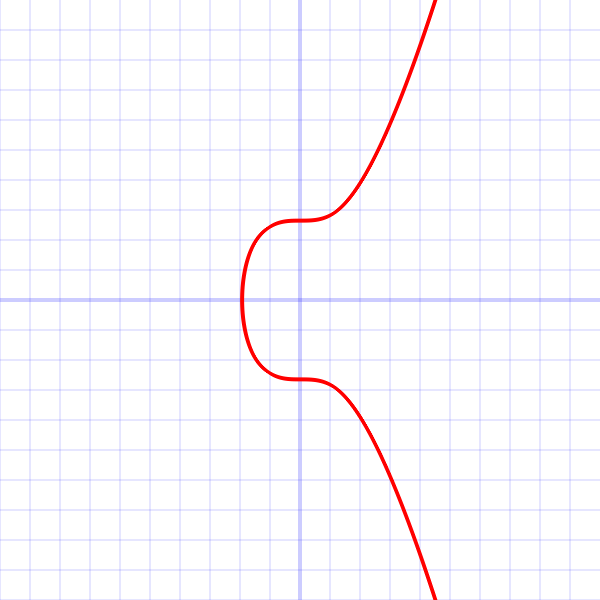
\includegraphics[width=0.5\textwidth]{introduction/images/Secp256k1.png}
	\caption{The \texttt{Secp256k1} plotted over real numbers. Note that the real
	curve is over a field, and thus looks more like a scattering of random points}
	\label{fig:eccbasic}
\end{figure}

The elliptic curve used can hold different parameters that defines it, certain
elliptic curves are standardized and have their own names. The curve used in
Bitcoin is named \texttt{Secp256k1}.\cite{Secp256k1_def}\cite{antonopoulos_2017}

The typical curve used in Elliptic curve cryptography is on the form
$y^2=x^3+ax+b$. The \texttt{Secp256k1} is defined with $a=0$ and $b=7$, making
the full \texttt{Secp256k1} equation: $y^2=x^3+7$. Which is plotted in figure
\ref*{fig:eccbasic}. For more in depth on elliptic curve cryptography see
section \ref{ecdsa}

%Mastering bitcoin
\Subsection{Blocks and the blockchain}
A block is fairly simple to understand, it is simply a datatype or structure
that holds information about itself, all the transactions that can fit and the
previous block in the chain (more on that in a bit). Because every block holds
information about the previous block you can follow all blocks backwards in time
all the way back to the original, also called the genesis block.\cite{genesis}
This is what is referred to as the blockchain.

A block could be added to the chain by anyone in the world. However it will only
be accepted if it has sufficient proof-of-work, and this is the key to how
consensus is reached in the network.\cite{antonopoulos_2017}

\begin{figure}[H]
	\centering
	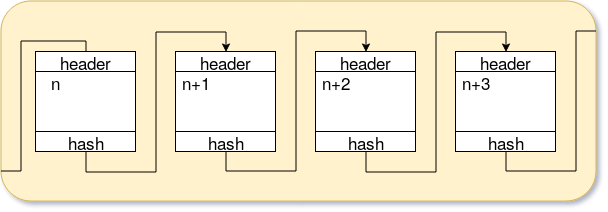
\includegraphics[width=0.5\textwidth]{introduction/images/blockchain.png}
	\caption{A basic overview of a blockchain}
	\label{fig:blockchain}
\end{figure}

\Subsubsection{Block-header}
Each block has a section of data called a header. The header contains meta-data 
about the block itself such as the version number, the id of the previous block 
in the chain, a timestamp of when the block was mined, the merkle root of 
all transactions (serves as proof of what transactions was included in the block) 
and a 32-bit field called nonce. 

The size of the header is always 80-bytes, a blocks id\footnote{Block id and 
block hash refers to the same thing. The terms might be mixed throughout the report.} 
is equal to the hash of its header. For example the genesis block in the 
Bitcoin blockchain has the id:

\texttt{000000000019d6689c085ae165831e934ff763ae46a2a6c172b3f1b60a8ce26f}

Something that you will find with all block-ids is that they always have leading zeroes. 
This is a side-effect  caused by mining and proof-of-work as explained in section \ref{intro-proof}.

%The section on SHA256 can be improved
\Subsection{Proof-of-work}\label{intro-proof}
Proof-of-work is, just like digital signatures, based in cryptographic
mathematics. Before we go on, you first need to understand what a hashing
algorithm does, the hashing algorithm used in Bitcoin is called \texttt{SHA256}.
\texttt{SHA256} takes in data of any size and produces a sort of finger print
of 256 bits.

For example the \texttt{SHA256} of the text ''cool'':

\fbox{\begin{minipage}{\textwidth}
	\texttt{echo "cool" | openssl sha256}
\end{minipage}}

Produces:

\fbox{\begin{minipage}{\textwidth}
		\texttt{27c16ce7e3861da034af1bb356d6a4f38cb84fa65d51fa62f69727143b4c6b60}
\end{minipage}}

The text produced is actually bytes represented in a hexadecimal number system,
in fact the entire string can be considered to be a very large number. Just like
with the digital signature there is no known viable way that can take a hash and
find what the original data that produced it was.

There is a term in Bitcoin called mining difficulty, or just difficulty. This
is a large number, 256 bits to be exact. When you want to add a new block to
the chain you have to do something called mining, this is a process where you
change the nonce-bits in the block-header until the id of the block (Think
of this as a number) is less than the target difficulty. The term hashpower refers
to how many times the machine you are using to mine blocks can test a certain
combination of variables per second, or H/s (Hashes per second).

The difficulty of mining a block is adjusted about every 2 weeks (every 2016th block to be exact). The difficulty
is calculated by each individual node whenever the block count is a multiple of 2016, the nodes go by the timestamps in the blocks, and should thus all reach the same conclusion. The new calculated difficulty is the one all the next 2016 blocks have to reach.\cite{antonopoulos_2017}

The accepted order of transactions is the order going backwards from the latest
block on the longest chain. The longest chain is always the one that the majority
is mining towards. What it basically
means is that as long as you trust 51\% of the participants in the network you
can also trust that the order of transactions is correct.\footnote{This is a simplification, but still holds true} This mechanism
prevents things like double spending the same money and holds a property called
emergent consensus, which means that eventually the entire network will agree
on the order of transactions.

In figure \ref{fig:blockchain2} is a diagram showing the longest chain, meaning
the chain with most proof of work. The block in green is the latest block on
that chain. The yellow block is what is known as a stale block, a block that is
part of the chain but not part of the longest chain of blocks. Transactions in
a stale block are not considered valid, and eventually they can be pruned
(deleted) because they do not effect the future in any way. A stale block occurs
if a new block is found in different parts of the network at almost the same
time. Then the network will be split, each node tries to find the next block on
the chain of whatever block they received first. In the case shown below the
chain on the left ''won'' and the green block is now the longest chain.

The red block in figure \ref{fig:blockchain2} is what is known as an orphan
block, that is, it has no known parent in the chain. This can happen if someone
mines a block that is malformed or when building the chain for a new node and
the blocks are received out of order.

\begin{figure}[H]
	\centering
	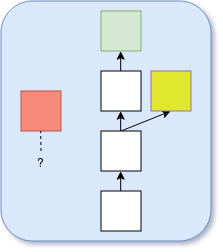
\includegraphics[width=0.2\textwidth]{introduction/images/more_blockchain.png}
	\caption{A diagram showing the longest chain, The green block is the latest
	block on the longest chain. The red block is a an orphan block, the yellow
	block is a stale block}
	\label{fig:blockchain2}
\end{figure}


\Subsection{Software}
Just like how you can use regular money without knowing the underlying process
and technology of banking systems for example, you can use Bitcoin without
knowing the details of how it works. There is plenty of software that handles
wallets, transactions etc for you.

%Removed for now
%A good example is mycelium wallet for Android.

\Subsection{Programmable transactions}
Another feature that Bitcoin has, which makes it very versatile, is that transactions are programmable.
As mentioned earlier the most
common transaction is sending the money to someones public key. What really
goes on here is that the person who wants to spend whatever money was sent to
them has to prove programmaticlly that they own the private key related to that
public key.

This is not the only type of transaction possible, Bitcoin has its own little
programming language called \texttt{Script}. Any type of transaction that can
be described in script is possible as a transaction. This is the basis for atomic swaps, payment channels and lightning network, which will be discussed in the following sections
